 % !TEX program = lualatex
\documentclass[xcolor={x11names, table}, compress]{beamer}

\usepackage{xcolor}
\usepackage{fontspec}
\usepackage{pgfplots}
\usepackage{tikz}
\usepackage{amsmath, amssymb, amsfonts}
\usepackage{bm}
\usepackage{eso-pic}
\usepackage{graphicx}

\pgfplotsset{compat=1.15}
\usetikzlibrary{positioning, shapes, calc, arrows}
\hypersetup{pdfstartview={Fit}}

%% Beamer Layout %%%%%%%%%%%%%%%%%%%%%%%%%%%%%%%%%%
\useinnertheme{default}
\usepackage[T1]{fontenc}
\usefonttheme{professionalfonts}

\setbeamerfont{frametitle}{}

\definecolor{BHKpresentationDark}{RGB}{114,133,176}
\definecolor{BHKpresentationDarkGrey}{RGB}{103,116,128}
\definecolor{BHKblue}{RGB}{51,105,153}

\setbeamerfont{title like}{shape=\scshape}
\setbeamercolor*{frametitle}{fg=BHKpresentationDark} 
\setbeamercolor*{lower separation line head}{bg=BHKblue} 
\setbeamercolor*{normal text}{fg=BHKpresentationDarkGrey,bg=white} 
\setbeamercolor*{alerted text}{fg=BHKblue} 
\setbeamercolor*{example text}{fg=black} 
\setbeamercolor*{item}{fg=BHKpresentationDark,bg=gray} 
\setbeamercolor{enumerate item}{fg=BHKpresentationDark}
\setbeamercolor*{structure}{fg=black} 
\setbeamercolor*{palette tertiary}{fg=black,bg=black!10} 
\setbeamercolor*{palette quaternary}{fg=black,bg=black!10} 
\setbeamercovered{transparent}

\setbeamertemplate{navigation symbols}{}
\setbeamertemplate{footline}{%
    \begin{beamercolorbox}[wd=\paperwidth]{footlinecolor}
        
\includegraphics[width=\textwidth]{bar_footline.pdf}
    \end{beamercolorbox}%
}

\setbeamertemplate{frametitle}[default][center]
\setbeamertemplate{caption}[numbered]
\setbeamertemplate{section in toc}[sections numbered]
\setbeamertemplate{subsection in toc}[subsections numbered]


\newcommand{\insertsec}{\thesection.~\insertsection}
\newcommand{\insertsubsec}{\thesection.\thesubsection~\insertsubsection}

%%%%%%%%%%%%%%%%%%%%%%%%%%%%%%%%%%%
%% Start of document %%%%%%%%%%%%%%
%%%%%%%%%%%%%%%%%%%%%%%%%%%%%%%%%%%

\begin{document}
%%%% title slide %%%%%
{\setbeamertemplate{footline}{} 
    \begin{frame}
        \vspace{-1.5cm}
        \hfill\makebox[0.2\paperwidth]{
\includegraphics[width=0.4\textwidth]{logo_wtext}}
        \begin{flushleft}
            \hspace{-1cm}
\includegraphics[width=0.8\textwidth, height=0.4em]{title_line.pdf}\hfill
            
            \title{
                \begin{flushleft}{\huge \color{BHKpresentationDark} 
                Convolutional Neural Networks Summary
            } 
            \end{flushleft}}
            
            \date{$~~$}
            \author[Joan]{\begin{flushleft}\vspace{-1cm} Joan Marcè i Igual\end{flushleft}}
            \titlepage
        \end{flushleft}
    \end{frame}
}

\begin{frame}{Table of Contents}
	\tableofcontents
\end{frame}

\section{Introduction}
\begin{frame}{\insertsec}
	\begin{itemize}
    \item Nowadays Machine Learning it's widely used
    \item Medical images can be obtained using MRI, PET or CT scans but are underused
    \item Different methods have appeared to analyze these data for image classification,
    object detection, segmentation...
    \item Deep learning models aim to be able to unlock the full potential of medical imaging
  \end{itemize}
\end{frame}

\subsection{Survival Analysis}
\begin{frame}{\insertsubsec}
  Survival analysis models usually have:
  \begin{itemize}
    \item Baseline data \( x \)
    \item Event \( E \in \{0, 1\} \)
    \item Time \( T \)
  \end{itemize}

  Casting the survival problem as a ranking is a way of dealing with censored data.
  \vspace{.3cm}
  \begin{columns}
    \begin{column}{.5\textwidth}
      \begin{figure}
        \centering
        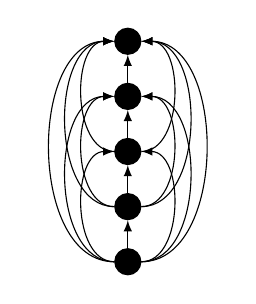
\begin{tikzpicture}[scale=.7]
  \tikzstyle{bDot}=[circle, fill=black, draw]
  \foreach \y in {1,...,5} {
    \node[bDot] (D-\y) at (0, \y) {};
  }

  \foreach \y in {1,...,4} {
    \pgfmathsetmacro{\z}{int(\y + 1)}
    \draw[-latex] (D-\y) -- ({D-\z}.south);
  }

  \foreach \y in {1,...,3} {
    \pgfmathsetmacro{\z}{int(\y + 2)}
    \foreach \j in {\z,...,5} {
      \ifthenelse{\y=2 \OR \y=3}{
        \draw[-latex] (D-\y) to[bend left=90] (D-\j);
      }{
        \draw[-latex] (D-\y) to[bend right=90] (D-\j);
      }
    }
  }
\end{tikzpicture}

        \caption{Uncensored data}
      \end{figure}
    \end{column}
    \begin{column}{.5\textwidth}
      \begin{figure}
        \centering
        \begin{tikzpicture}
  \foreach \y in {1,...,5} {
    \ifthenelse{\y=2 \OR \y=4}{
      \node [circle, fill=white, draw=black] (D-\y) at (0, \y) {};
    }{
      \node [circle, fill=black, draw=black] (D-\y) at (0, \y) {};
    }

    \foreach \y in {3,4,5} {
      \draw [-latex] (D-1) to[bend right=90] (D-\y);
    }

    \foreach \y/\z in {1/2, 3/4} {
      \draw [-latex] (D-\y) -- (D-\z);
    }
    \draw [-latex] (D-3) to[bend left=90] (D-5);
  }
\end{tikzpicture}

        \caption{Censored data}
      \end{figure}
    \end{column}
  \end{columns}
  
\end{frame} 
\section{Neural Networks}
\begin{frame}{\insertsec}
	
\tikzset{
  pics/layer/.style n args = {3}{
    code = {
      \foreach \y in {1,...,#1} {
        \node[draw, circle] (L-#2-\y) at (0,{1.5*(\y - #1/2)}) {${#3}_{#2 \y}$};
      }
    }
  }
}

\begin{tikzpicture}
\def\layers{2/I, 5/H, 5/H, 3/O}

\foreach \x/\name [count=\xi] in \layers  {
  \draw (3*\xi, 0) pic {layer={\x}{\xi}{\name}};
}

\foreach \x/\ignore [count=\xi, remember=\xi as \lastxi, remember=\x as \lastx] in \layers {
  \ifthenelse{\xi > 1}{
    \foreach \ylast in {1,...,\lastx} \foreach \y in {1,...,\x}{
      \draw [-latex] (L-\lastxi-\ylast) -- (L-\xi-\y);
    }
  }{};
}

\end{tikzpicture}


\end{frame}

\subsection{Parameters}
\begin{frame}{\insertsubsec}
    \begin{columns}[t]
        \column{.6\textwidth}
        \begin{itemize}
            \item $l$: Current layer
            \item $w_{i, j}^{[l]}$: Weight from unit $j$ to $i$ at layer $l$
            \item $b_{i}^{[l]}$: Bias for unit $i$ at layer $l$
            \item $n^{[l]}$: Number of units in layer $l$
            \item $\bm{W}^{[l]} \in \mathbb{R}^{n^{[l]} \times n^{[l - 1]}}$: Weight matrix
            \item $\bm{b}^{[l]} \in \mathbb{R}^{n^{[l]}}$: Bias
            \item $
            \begin{aligned}[t]
            \bm{a}^{[l]} &= g(\bm{W}^{[l]}\cdot \bm{a}^{[l - 1]} + \bm{b}^{[l]}) \\
            \bm{a}^{[l]} &\in \mathbb{R}^{n^{[l]}}
            \end{aligned}
            $ Activations for layer $l$
            \item $g(x)$: Activation function
        \end{itemize}
        \column{.5\textwidth}
        \centering
        \begin{columns}[t]
    \column{.5\textwidth}
    \centering
    \begin{figure}
        \begin{tikzpicture}
            \begin{axis}[
                width=\textwidth,
                height=.8\textwidth,
                grid=major,
                grid style={dashed, gray!30},
                xtick={-5, 0, 5},
                xticklabels={$-\infty$, $0$, $+\infty$}
                ]
                \addplot[mark=none]{tanh(x)};
            \end{axis}
        \end{tikzpicture}
        \caption{$\tanh(x)$}
    \end{figure}
    \centering
    \column{.5\textwidth}
    \begin{figure}
        \begin{tikzpicture}
            \begin{axis}[
                width=\textwidth,
                height=.8\textwidth,
                grid=major,
                grid style={dashed, gray!30},
                xtick={-5, 0, 5},
                xticklabels={\empty, $0$, \empty}
                ]
                \addplot[mark=none]{max(x, 0)};
            \end{axis}
        \end{tikzpicture}
        \caption{ReLU function}
    \end{figure}
\end{columns}
    \end{columns}
\end{frame}
\begin{frame}
    \begin{columns}
        \column{.6\textwidth}
        \begin{block}{Cost function}
            $$
            J(\bm{W}, \bm{b}, \hat{\bm{y}}, \bm{y}) = 
            \frac{1}{m} \sum_{i=1}^{m} \mathcal{L}(\hat{\bm{y}}^{(i)}, \bm{y}^{(i)})
            $$
        \end{block}
        \begin{block}{Loss function}
            $$
            \mathcal{L}(\hat{\bm{y}}, \bm{y}) = ||\hat{\bm{y}} - \bm{y}||^2
            $$
        \end{block}
        \begin{block}{Parameters update}
            \begin{align*}
            \bm{W} &:= \bm{W} - \alpha \cdot \frac{\partial J}{\partial \bm{W}} \\
            \bm{b} &:= \bm{b} - \alpha \cdot \frac{\partial J}{\partial \bm{b}}
            \end{align*}
        \end{block}
        \column{.4\textwidth}
        To achieve better results at predicting $\hat{\bm{y}}$ 
        we have to minimize the cost function $J(\bm{W}, \bm{b}, \hat{\bm{y}}, \bm{y})$.
    \end{columns}
\end{frame}
\section{Convolutional Neural Networks}
\begin{frame}{\insertsec}
    This type of networks are a bit different because instead of computing the activations by
    multiplying the previous ones with the weight matrix it convolutes the previous activations 
    (denoted by $*$):
    
    \begin{align*}
        \bm{a}^{[l]} &= g(\bm{W}^{[l]}\cdot \bm{a}^{[l - 1]} + \bm{b}^{[l]}) \\
        \text{Becomes:} \\
        \bm{a}^{[l]} &= g(\bm{W}^{[l]} * \bm{a}^{[l-1]} + \bm{b}^{[l]})
    \end{align*}
\end{frame}

\subsection{Convolution Operation}
\begin{frame}{\insertsubsec}
    \begin{alertblock}{Important}
        What we call \textit{Convolution} in ML it's actually the \textit{Cross-Correlation} operation
        in signal analysis.
    \end{alertblock}
    
    \begin{align*}
        \left(
        \begin{array}{cccccc}
            10 & \cellcolor{green!20}10 & \cellcolor{green!20}10 & \cellcolor{green!20}0 & 0 & 0 \\
            10 & \cellcolor{green!20}10 & \cellcolor{green!20}10 & \cellcolor{green!20}0 & 0 & 0 \\
            10 & \cellcolor{green!20}10 & \cellcolor{green!20}10 & \cellcolor{green!20}0 & 0 & 0 \\
            10 & 10 & 10 & 0 & 0 & 0 \\
            10 & 10 & 10 & 0 & 0 & 0 \\
            10 & 10 & 10 & 0 & 0 & 0 \\
        \end{array}
        \right)
        *
        \left(
        \begin{array}{ccc}
            1 & 0 & -1 \\
            1 & 0 & -1 \\ 
            1 & 0 & -1 \\
        \end{array}
        \right)
        = 
        \left(
        \begin{array}{cccc}
            0 & \cellcolor{green!20}30 & 30 & 0 \\
            0 & 30 & 30 & 0 \\
            0 & 30 & 30 & 0 \\
            0 & 30 & 30 & 0 \\
        \end{array}
        \right)
    \end{align*}
    $$
        10 \cdot 1 + 10 \cdot 1 + 10 \cdot 1 +
        10 \cdot 0 + 10 \cdot 0 + 10 \cdot 0 +
        0 \cdot -1 + 0 \cdot -1 + 0 \cdot -1 = 30
    $$
\end{frame}

\begin{frame}
    With convolutions the Neural Network parameters ($w$) are the convolution matrix elements
    and so we do multiple convolutions to filter different features.
    

\begin{figure}[H]
    \tikzset{pics/3DBox/.style n args={3}{code={
        \tikzstyle{box}=[blue, fill=blue!20];
        \draw[box] (0, 0, 0) -- (0, #2, 0) -- (#1, #2, 0) -- (#1, 0, 0) -- cycle;
        \draw[box] (#1, 0, 0) -- (#1, 0, -#3) -- (#1, #2, -#3) -- (#1, #2, 0) -- cycle;
        \draw[box] (0, #2, 0) -- (#1, #2, 0) -- (#1, #2, -#3) -- (0, #2, -#3) -- cycle; 
    }}}

    \begin{tikzpicture}
        \path pic at (0, 0, 0) {3DBox={2}{2}{1}};
        \path pic at (6, .5, 1) {3DBox={1}{1}{3}};
        \draw [-latex] (3, 1, 0) -- (5, 1, 0) node[above, midway] {$5 \times 5$ filter};

        \node [anchor=west] at (0, -1, 0) {$(64 \times 64 \times 3)$};
        \node [anchor=west] at (5 , -1, 0) {$(60 \times 60 \times 10)$};
    \end{tikzpicture}
\end{figure}


\end{frame}

\subsection{Pooling operation}
\begin{frame}{\insertsubsec}
    We use pooling to reduce the volume width and height size
    \begin{block}{Max-Pooling}
        \begin{align*}
            \operatorname{max\,pool}
            \left(
            \begin{array}{cccc}
                \cellcolor{green!20} 0 & \cellcolor{green!20} 7 & 12 &  9 \\
                \cellcolor{green!20}15 & \cellcolor{green!20} 3 & 22 &  6 \\
                 2 & 12 &  8 &  3 \\
                 6 &  2 & 18 &  3 \\
            \end{array}
            \right)
            =
            \left(
            \begin{array}{cc}
                \cellcolor{green!20}15 & 22 \\
                12 & 18
            \end{array}
            \right)
        \end{align*}
    \end{block}

    \begin{block}{Avg-Pooling}
        \begin{align*}
            \operatorname{avg\,pool}
            \left(
            \begin{array}{cccc}
                \cellcolor{green!20} 0 & \cellcolor{green!20} 7 & 12 &  9 \\
                \cellcolor{green!20}15 & \cellcolor{green!20} 3 & 22 &  6 \\
                 2 & 12 &  8 &  3 \\
                 6 &  2 & 18 &  3 \\
            \end{array}
            \right)
            =
            \left(
            \begin{array}{cc}
                \cellcolor{green!20}6.25 & 12.25 \\
                5.50 & 8.00
            \end{array}
            \right)
        \end{align*}
    \end{block}
\end{frame}

\subsection{Residual Networks}
\begin{frame}{\insertsubsec}
    They are a type of network that can learn the identity function thus allowing us to do
    very deep networks.
    \def\layersep{1.5cm}

\begin{figure}[H]
    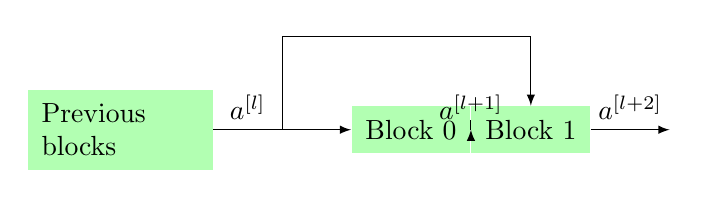
\begin{tikzpicture}[node distance=\layersep]
        \tikzstyle{block}=[rectangle, fill=green!30, inner sep = 5pt]
        \node[block] (R0) at (0, 0) {Block 0};
        \node[left = .75 of R0] (A0) {};
        \node[above = .75 of R0] (A1) {};
        \node[block, left = .75 of A0, text width = 2cm] (I0) {Previous blocks};
        \node[block, right = of R0] (R1) {Block 1};
        \node[right = 1 of R1] (A2) {};

        % Arrows
        \draw [-latex] (I0) -- (R0) node[above, near start] {$a^{[l]}$};
        \draw [-latex] (R0) -- (R1) node[above, midway] {$a^{[l + 1]}$};
        \draw (A0.center) |- (A1.center); 
        \draw [-latex] (A1.center) -| (R1.north);
        \draw [-latex] (R1) -- (A2) node[above, midway] {$a^{[l + 2]}$};
    \end{tikzpicture}
\end{figure}

    \begin{align*}
        \bm{a}^{[l+2]} = 
        g(\underbrace{W^{[l+2]} \cdot \bm{a}^{[l + 1]} + \bm{b}^{[l + 2]}}
        _{0 \text{ if using regularization}} + \bm{a}^{[l]})
    \end{align*}
\end{frame}

\subsection{Inception block}
\begin{frame}{\insertsubsec}
    \begin{figure}[H]
        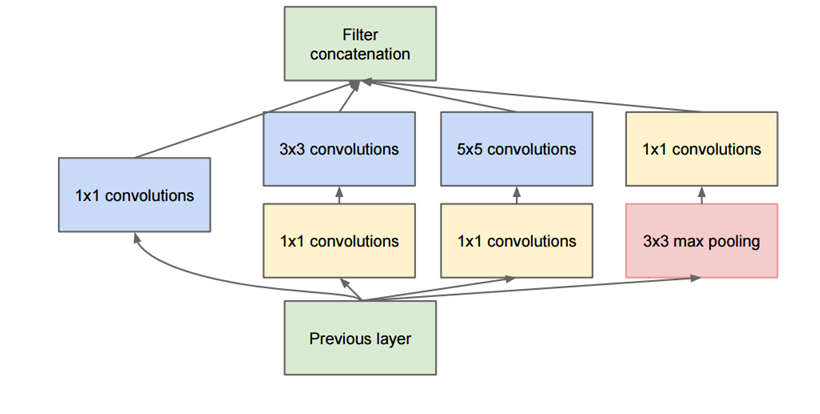
\includegraphics[width=\textwidth]{images/GoogLeNet3}
        \caption{GoogLeNet Inception Module}
    \end{figure}
\end{frame}






\end{document}